\documentclass{article}

\usepackage{pdflscape}
\usepackage{pgf}
\usepackage{tikz}
\usetikzlibrary{arrows,automata}
\usepackage[latin1]{inputenc}
\begin{document}
	\pagenumbering{gobble}
	
	\begin{landscape}
	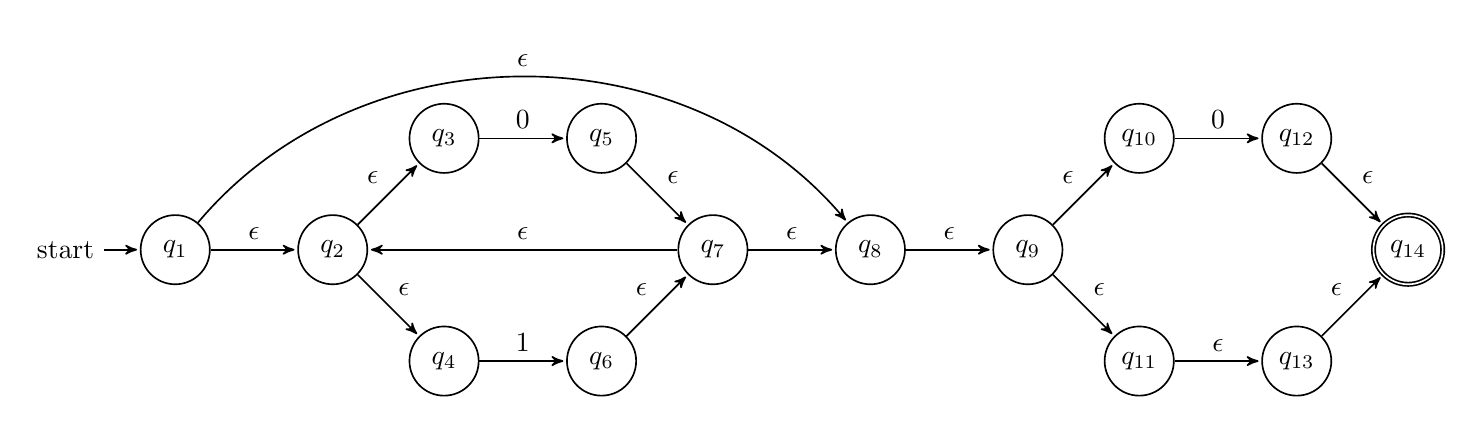
\begin{tikzpicture}[->,>=stealth',shorten >=1pt,auto,node distance=2cm,
	semithick]
	\tikzstyle{every state}=[fill=none,draw=#1,text=black]
	
	\node[initial,state] (A)    {$q_{1}$};
	\node[state]          (B) [right of=A] {$q_{2}$};
	\node[state]          (C) [above right of=B] {$q_{3}$};
	\node[state]          (D) [below right of=B] {$q_{4}$};
	\node[state]          (E) [right of=C] {$q_{5}$};
	\node[state]          (F) [right of=D] {$q_{6}$};
	\node[state]          (G) [below right of=E] {$q_{7}$};
	\node[state]          (H) [right of=G] {$q_{8}$};
	\node[state]          (I) [right of=H] {$q_{9}$};
	
	\node[state]          (J) [above right of=I] {$q_{10}$};
	\node[state]          (K) [below right of=I] {$q_{11}$};
	
	\node[state]          (L) [right of=J] {$q_{12}$};
	\node[state]          (M) [right of=K] {$q_{13}$};
	
	\node[state, accepting]          (O) [below right of=L] {$q_{14}$};
	
	
	
	\path (A) edge [left, above]      node {$\epsilon$} (B);
	\path (A) edge [bend left=50]      node {$\epsilon$} (H);
	\path (B) edge node {$\epsilon$} (C);
	\path (B) edge node {$\epsilon$} (D);
	
	\path (C) edge node {$0$} (E);
	\path (D) edge node {$1$} (F);
	
	\path (E) edge node {$\epsilon$} (G);
	\path (F) edge node {$\epsilon$} (G);
	
	\path (G) edge node {$\epsilon$} (H);
	\path (G) edge [left, above] node {$\epsilon$} (B);
	
	\path (H) edge node {$\epsilon$} (I);
	
	\path (I) edge node {$\epsilon$} (J);
	\path (I) edge node {$\epsilon$} (K);
	
	
	\path (J) edge node {$0$} (L);
	\path (K) edge node {$\epsilon$} (M);
	
	
	\path (L) edge node {$\epsilon$} (O);
	\path (M) edge node {$\epsilon$} (O);
	
	
	\end{tikzpicture}
	
	\end{landscape}
	
\end{document}